\documentclass[../../main.tex]{subfiles}
\begin{document}

\begin{flushright}
  \footnotesize\textit{【自動文字起こし・要確認】}
\end{flushright}

% Source: handwritten.pdf 第3問．
% 原稿p.4の見出しは「第4問」だが，内容は乙第3問に対応する．
$c=\cos x$，$s=\sin x$と略記する．まず
\begin{align}
  S=\int_0^\pi\sin x\,dx=2.
\end{align}
$y=\sin x$と$y=a\cos x$の交点の$x$座標を$\alpha$とすると，$0<\alpha<\dfrac{\pi}{2}$で
\begin{align}
  \sin\alpha=a\cos\alpha.
\end{align}
また
\begin{align}
  T&=\int_0^\alpha\sin x\,dx+\int_\alpha^{\pi/2}a\cos x\,dx\\
  &=1-\cos\alpha+a(1-\sin\alpha).
\end{align}
$S:T=3:1$より
\begin{align}
  0&=1-3\cos\alpha+3a(1-\sin\alpha).
\end{align}
$a=\dfrac{\sin\alpha}{\cos\alpha}$を代入して
\begin{align}
  0&=(1-3\cos\alpha)\cos\alpha+3\sin\alpha(1-\sin\alpha),\\
  3&=\cos\alpha+3\sin\alpha.
\end{align}
$t=\tan\dfrac{\alpha}{2}$とおけば
\begin{align}
  \cos\alpha=\dfrac{1-t^2}{1+t^2},\qquad \sin\alpha=\dfrac{2t}{1+t^2},
\end{align}
だから
\begin{align}
  3(1+t^2)&=1-t^2+6t,\\
  4t^2-6t+2&=0,\\
  (2t-1)(t-1)&=0.
\end{align}
$0<t<1$より$t=\dfrac{1}{2}$．したがって
\begin{align}
  a=\tan\alpha=\dfrac{2t}{1-t^2}=\dfrac{1}{1-\dfrac{1}{4}}=\dfrac{4}{3}.
\end{align}
\paragraph{解2}
$a=\tan\alpha$，$0<\alpha<\dfrac{\pi}{2}$だから
\begin{align}
  \sin\alpha=\dfrac{a}{\sqrt{a^2+1}},\qquad \cos\alpha=\dfrac{1}{\sqrt{a^2+1}}.
\end{align}
これらを$S:T=3:1$の式に代入しても$a=\dfrac{4}{3}$を得る．
\begin{figure}[H]
  \begin{center}
    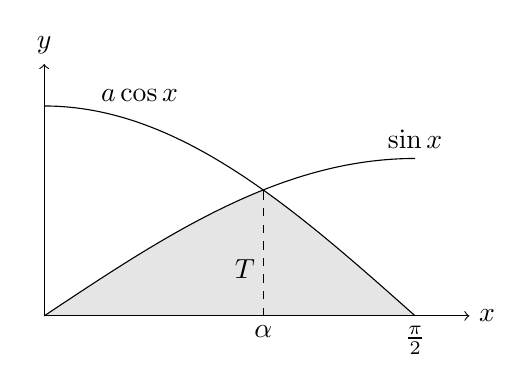
\begin{tikzpicture}[xscale=3,yscale=2]
      \fill[gray!20] (0,0)--plot[domain=0:.9273,samples=50](\x,{sin(\x r)})--plot[domain=.9273:1.5708,samples=50](\x,{4*cos(\x r)/3})--cycle;
      \draw[->] (0,0)--(1.8,0) node[right]{$x$};\draw[->] (0,0)--(0,1.6) node[above]{$y$};
      \draw plot[domain=0:1.5708,samples=60](\x,{sin(\x r)}) node[above]{$\sin x$};
      \draw plot[domain=0:1.5708,samples=60](\x,{4*cos(\x r)/3});\node[right] at (.2,1.4){$a\cos x$};
      \draw[dashed] (.9273,0) node[below]{$\alpha$}--(.9273,.8);\node[below] at (1.5708,0){$\frac{\pi}{2}$};\node at (.85,.3){$T$};
    \end{tikzpicture}
  \end{center}
  \caption{二つの曲線と$x$軸で囲まれる領域}
\end{figure}

\end{document}
